\section{Overapproximation of Synchronous Traces} \label{sec:approach}
\alert{TODO: summary. main idea is to reduce bookkeeping as much as possible to improve scalability. note we use bool signals for convenience of demonstration, but the methods are general unless otherwise stated.}

STL$^+$ has the same syntax as STL and the below semantics.
$\tr^+(S,{\hb})$ is the overapproximation we compute.

\small
\begin{equation*}
	[(S,{\hb}) \models \varphi]_{\mathsf{STL}^+} = 
	\begin{cases}
		\top & \text{ if } \forall w \in \tr^+(S,{\hb}) : [w \models \varphi]_{\mathsf{STL}} \\
		\bot & \text{ if } \forall w \in \tr^+(S,{\hb}) : [w \models \lnot\varphi]_{\mathsf{STL}} \\
		\,? & \text{ otherwise}
	\end{cases}
\end{equation*}
\normalsize

\begin{theorem}
	For every STL formula $\varphi$ and every distributed signal $(S,{\hb})$, if $[(S,{\hb}) \models \varphi]_{\mathsf{STL}^+}$ then $[(S,{\hb}) \models \varphi]_{\mathsf{STL}}$.
\end{theorem}

\subsection{Uncertainty Regions and Canonical Segmentations}

Consider a signal $x : [0,d) \to \B$ with a rising edge at local time $t$.
Due to clock skew, the rising edge of $x$ occurs in the range $(t - \varepsilon, t + \varepsilon)$ according to the global clock.
This range is called an \emph{uncertainty region} because in the interval $(t - \varepsilon, t + \varepsilon)$ the monitor cannot tell the value of $x$ precisely, but only that it changes from $\bot$ to $\top$.
To systematically reason about this uncertainty, we use the notion of segmentation of temporal domains of signals.

Given a temporal domain $I = [0,d) \subset \R_{\geq 0}$, a \emph{segmentation} of $I$ is a partition of $I$ into finitely many intervals $I_1, \ldots, I_k$ of the form $I_j = [t_j, t_{j+1})$ such that $t_j < t_{j+1}$ for all $1 \leq j \leq k$.
By extension, a segmentation of a collection of signals with the same temporal domain $I$ is a segmentation of $I$.

Let $x : [0,d) \to \R$ be a signal and $(t, x(t))$ be an edge of $x$. %$E_x = \{(t_1, x(t_1)), \ldots, (t_m, x(t_m))\}$ be the set of edges of $x$, given in an increasing order of local clock values.
We define $\theta_{\text{lo}}(x,t) = \max(0, t - \varepsilon)$ and $\theta_{\text{hi}}(x,t) = t_i + \varepsilon$.
%\begin{align*}
%	%	\theta_{\text{lo}}(x,t_i) &= \max\{0, \max_{j \in \{1, i\}} t_j - \varepsilon - (j-i)\delta\} \text{, and} \\
%	\theta_{\text{lo}}(x,t_i) &= \max_{1 \leq j \leq i} t_j - \varepsilon + (i-j)\delta \text{, and} \\
%	\theta_{\text{hi}}(x,t_i) &= \min_{i \leq j \leq m} t_j + \varepsilon - (j-i)\delta.
%\end{align*}
Intuitively, $\theta_{\text{lo}}$ and $\theta_{\text{hi}}$ give us the lower and upper bounds on the value of the monitor's clock for a given edge, i.e., the end points of the uncertainty region of the given edge.
We use these to describe a canonical segmentation of a distributed signal.

Let $(S,{\hb})$ be a distributed signal of $n$ signals.
For each signal $x_i$, let $F_i$ be the set of end points of its uncertainty regions.
Let $d' = \max(d, \max (\bigcup_{i = 1}^{n} F_i))$, which corresponds to the duration of the distributed signal with respect to the monitor's clock.
%
We define $F = \{0, d'\} \cup \bigcup_{i = 1}^{n} F_i$ and let $(a_j)_{1 \leq j \leq |F|}$ be a nondecreasing sequence of clock values corresponding to the elements of $F$.
Then, the \emph{canonical segmentation} of $(S,{\hb})$ is $G_S = \{I_1, \ldots, I_{|F| - 1}\}$ where $I_j = [a_j, a_{j+1})$ for all $1 \leq j < |F|$.
We present an example in \cref{fig:???}

%\begin{example} \label{ex:canonseg}
%	Let $(S, {\hb})$ be a distributed signal with $S = (x_1, x_2)$ over the temporal domain $[0,8)$ such that $\pi(x_1) \neq \pi(x_2)$.\borzoo{$\pi$ is unnecessary.}
%	Suppose $x_1(0) = 2$ and $x_2(0) = 3$, and let $\varepsilon = 2$ and $\delta = 3$.	
%	Consider the case where $x_1$ has a rising edge $(3,5)$ and a falling edge $(5,3)$ while $x_2$ has a rising edge $(2,7)$ and a falling edge $(5,2)$.
%	For $x_1$, taking into account only the clock skew would give us the uncertainty regions $(1,5)$ and $(3,7)$.\borzoo{We should this by a figure.}
%	However, the computation of uncertainty regions take into account also the bounded variability.
%	Intuitively, if the rising edge of $x_1$ occurs at global time 1, considering bounded variability, its falling edge occurs at the earliest at global time 4 instead of 3.
%	Conversely, if the falling edge occurs at global time 7 then its rising edge occurs at the latest at global time 4 instead of 5.
%	Then, we obtain $F_1 = \{1, 4, 7\}$.
%	For $x_2$, the uncertainty regions are $(0,4)$ and $(3,7)$, which gives us $F_2 = \{0, 3, 4, 7\}$; and therefore, $F_S = \{0, 1, 3, 4, 7, 8\}$.
%	This leads to the canonical segmentation $G_S = \{[0,1), [1,3) ,[3,4) ,[4,7) ,[7,8)\}$.		
%\end{example}

\begin{figure} 
	\centering
	\caption{\alert{TODO}}
%	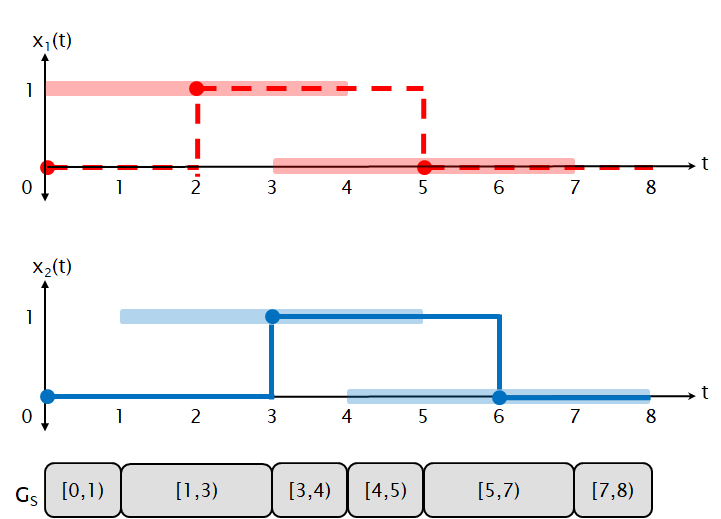
\includegraphics[scale=0.45]{canonseg.png}
%	\caption{The values of $x_1$ (solid) and $x_2$ (dashed) over time. The edges are marked with black balls and their uncertainty regions are given as light gray boxes around the edges. The resulting canonical segmentation $G_S$ is shown below the graphical representation of the signals.\label{fig:canonseg}}
\end{figure}


\subsection{Value Expressions}
\alert{TODO}

\subsection{Overapproximate Evaluation}
\alert{TODO -- for each signal concat the valexpr sets. choose one elt from each. stutter to the right length. this belongs to the set.}

